\documentclass{beamer}

\usepackage{listings}
\usepackage{tabulary}
\usepackage{amsmath}
\usepackage[utf8]{inputenc}
\usetheme{Madrid}
\setbeamersize{text margin left=0.1\textwidth,text margin right=0.1\textwidth}
\setbeamertemplate{section in toc}{\inserttocsection}
\lstset{language=python,
        keywordstyle=\color{red},
        basicstyle=\ttfamily,
        basicstyle=\small,
        frame = single,
        framexleftmargin=15pt,
        numbers=left,
        numberstyle=\small,
        numbersep=5pt,
        xleftmargin=0.05\textwidth,
        columns=fullflexible}
\definecolor{dgreen}{rgb}{0.,0.6,0.}
\definecolor{goldenrod}{rgb}{.9,0.6,0.1}

%Information to be included in the title page:
\title{Bayesian A/B Testing}
\subtitle{Conjugate Priors}
\author{Cary Goltermann}
\institute{Galvanize}
\date{2016}

 \AtBeginSubsection[]
{
  \begin{frame}
    \frametitle{Overview}
    \tableofcontents[currentsection,currentsubsection]
  \end{frame}
}

\begin{document}

\frame{\titlepage}

\begin{frame}
  \frametitle{Overview}
  \tableofcontents[]
\end{frame}

\section{A/B Testing}
\subsection{Frequentist - Review}
\begin{frame}
  \frametitle{Frequentist - Hypothesis Testing}
  \begin{tabulary}{\textwidth}{LL}
    \textcolor{blue}{Define a Metric} & Declare null and alternative hypothesis. \\ [2mm]
    \textcolor{blue}{Set Parameters} & Significance, number of observations, etc. \\ [2mm]
    \textcolor{blue}{Run Experiment} & Make sure you follow it to a tee. \\ [2mm]
    \textcolor{blue}{Compute Test Statistic} & Make sure it's the approprite one. \\ [7mm]
    \textcolor{blue}{Calculate P-Value} & \\ [2mm]
    \textcolor{blue}{Draw Conclusions} & Reject $H_0$ in favor of $H_A$, or fail to reject. \\ [2mm]
  \end{tabulary}
\end{frame}

\begin{frame}
  \frametitle{Frequentist A/B Testing - Limitations?}
  \begin{itemize}
    \item If one of the pages your testing appears to be obviously better, can you scrap the experiment and declare it the winner?
    \item At the end of an experiments, can you quantify how much better the winning pages is than the loosing page?
      \begin{columns}
        \column{0.8\textwidth}
        \begin{block}{Example}
          ``It's 95\% likely that page A is better than page B.''
        \end{block}
        \vspace{2mm}
      \end{columns}
    \item If, after you've begin your test, your boss comes to you with another version of the page and asks you to test it it too, can you update the test?
  \end{itemize}
\end{frame}

\subsection{Bayesian - Overview}
\begin{frame}
  \frametitle{Bayesian - Overview}
  \begin{tabulary}{\textwidth}{LL}
    \textcolor{blue}{Define a Metric} & To quantify what "better" means. \\ [2mm]
    \textcolor{blue}{Run Test} & Collect data. \\ [2mm]
    \textcolor{blue}{Continually Monitor Results} & Can decide to stop at any time. \\ [7mm]
    \textcolor{blue}{Suggest Next Step} & Based on probabilities calculated. \\ [2mm]
  \end{tabulary}
\end{frame}

\section{Bayesian A/B Testing}
\subsection{Bayes' Theorem}
\begin{frame}
  \frametitle{Bayes' Theorem}
  \begin{columns}
    \column{0.5\textwidth}
    \begin{block}{}
      \centering
      {\LARGE \textbf{$ P(\theta | y) = \frac{P(y | \theta) \times P(\theta)}{P(y)} $}}
    \end{block}
    \column{0.5\textwidth}
    \begin{description}
      \item[$ P(y | \theta) $] Likelihood
      \item[$ P(\theta) $] Prior
      \item[$ P(y) $] Normalizing Constant
    \end{description}
  \end{columns}
  \vspace{2mm}

  \begin{center}
    \textit{Remember: $ P(y) = \int P(y, \theta) d\theta $}
  \end{center}
  \vspace{4mm}
  \pause

  This equation captures the essence of Bayesian modeling: that the uncertainty about some unknown parameter can be quantified.
\end{frame}

\begin{frame}
  \frametitle{Bayes' Theorem Distilled}
  All that mathiness can be boiled down to the straightforward idea that:
  \vspace{4mm}

  \centering
  {\LARGE $ Posterior \propto Likelihood \times Prior $}
\end{frame}

\begin{frame}
  \frametitle{Back to A/B Testing}
  How, then, do we apply this supposedly straightforward idea of Bayes' Theorem to our statistics based question of A/B testing?
  \vspace{3mm}

  Let's first consider what we are really trying to do in the process of A/B testing. \vspace{3mm}
  \pause

  \begin{columns}
  \column{0.9\textwidth}
    \begin{block}{}
      Trying to determine which of options A \& B is "better".
    \end{block}
  \end{columns}

  \vspace{6mm}
  \pause
  For example, trying to determine which page layout has a higher click-through rate.
\end{frame}

\begin{frame}
  \frametitle{Moving Towards Bayes}
  Considering that distilled version of Bayes' Theorem we saw earlier:

  \begin{center}
    {\large $ Posterior \propto Likelihood \times Prior $}
  \end{center}
  \vspace{2mm}
  \pause

  Let's attach some tangible ideas to these abstract notions of a "likelihood" and a "posterior" for the click-through rate example. For the next two slides let's consider the data associated with each of our pages separately.
\end{frame}

\subsection{Likelihood}
\begin{frame}
  \frametitle{Likelihood}
  {\large What are the possible outcomes for each observation in our data for a single page?}
  \pause
  \vspace{1mm}

  \begin{center}
    A click-through occurs or not, binary result.
  \end{center}
  \pause
  \noindent\hfil\rule{\textwidth}{.4pt}\hfil

  \vspace{6mm}
  {\large How, then, are our data distributed; aka, what is the \textbf{likelihood}?}
  \pause
  \vspace{1mm}

  \begin{columns}
    \column{0.5\textwidth}
    \begin{block}{Binomial}
      $ P(X\! =\! k) = {{n}\choose{k}}\: p^k \times (1-p)^{n-k} $

      $\quad\rightarrow k$ successes in $n$ trials.
    \end{block}
  \end{columns}
\end{frame}

\subsection{Posterior}
\begin{frame}
  \frametitle{Posterior}
  {\large Again, with respect to the data from a single page, what are the possible values that a click-through rate can take on?}
  \pause
  \begin{center}
    Any real value in the open interval $ [0, 1] $.
  \end{center}
  \pause
  \vspace{-2mm}
  \noindent\hfil\rule{\textwidth}{.4pt}\hfil
  \vspace{3mm}

  {\large What distribution, then, should we use to model this click-through rate parameter; aka, what is the \textbf{posterior}?}
  \pause

  \begin{center}
    \textbf{Beta}! Has support over the continuous interval $ [0, 1] $.
  \vspace{-2mm}
  \end{center}
  \begin{columns}
    \column{0.65\textwidth}
    \begin{block}{Beta}
      $ X \sim Be(\alpha, \beta) = \frac{1}{B(\alpha, \beta)} x^{\alpha-1}(1-x)^{\beta-1} $
    \end{block}
  \end{columns}
\end{frame}

\begin{frame}
  \frametitle{Beta Distribution}
  \begin{columns}
    \column{0.8\textwidth}
      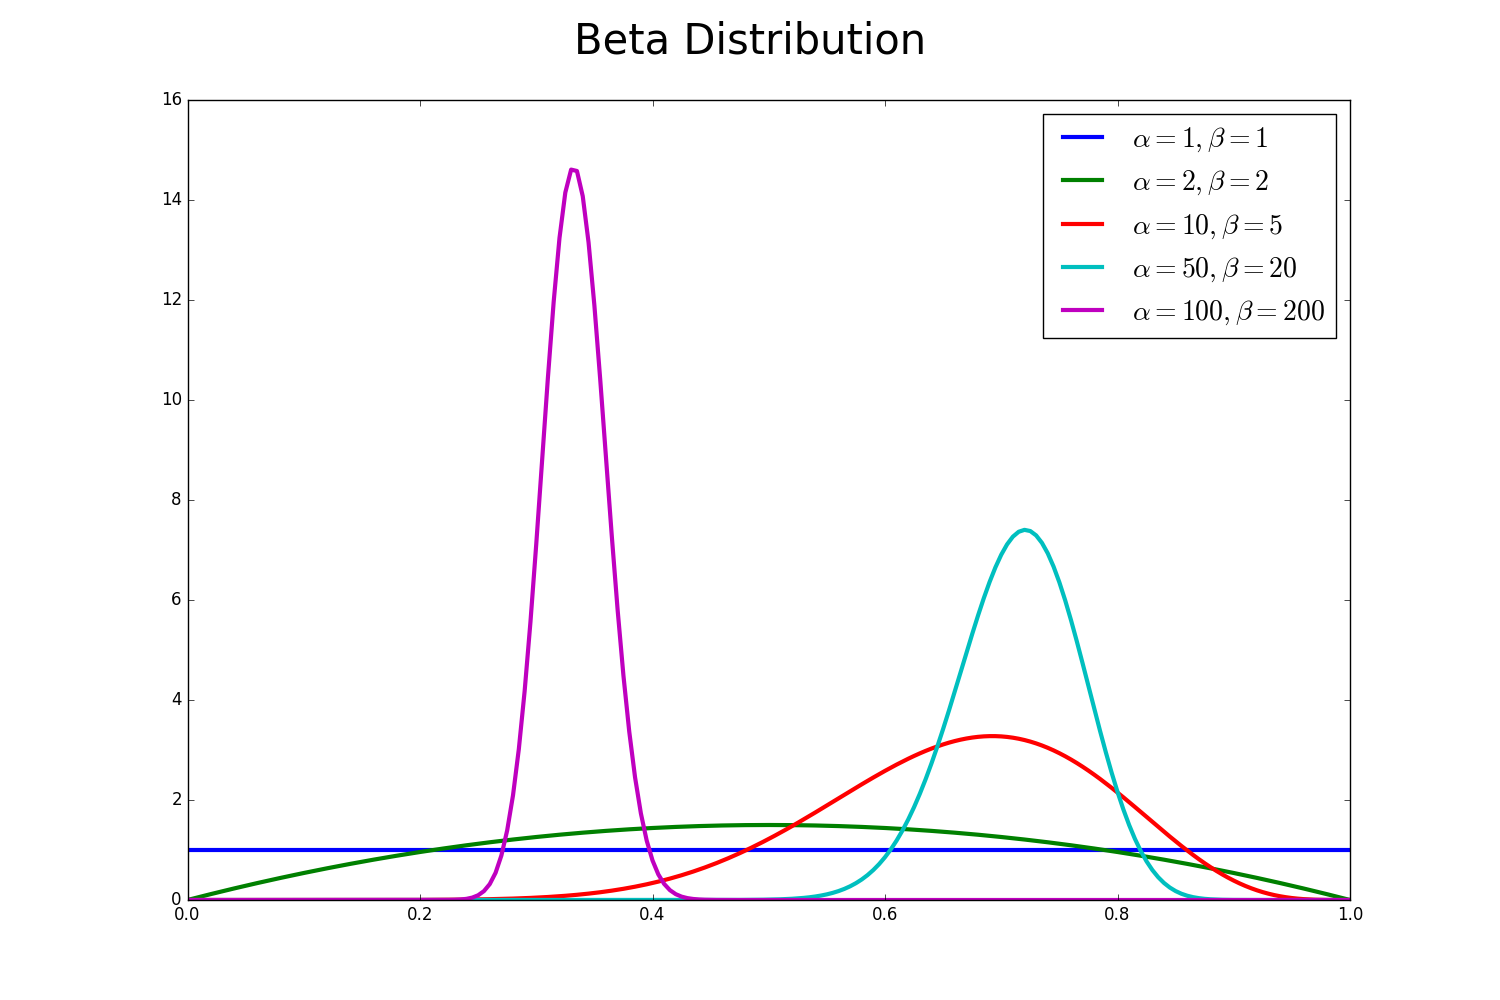
\includegraphics[width=\textwidth]{images/betas.png}
    \begin{columns}
      \column{0.5\textwidth}
        \centering
        $E[X] = \frac{\alpha}{\alpha+\beta}$
      \column{0.5\textwidth}
        \centering
        $Mode = \frac{\alpha-1}{\alpha+\beta-2}$
    \end{columns}
  \end{columns}
\end{frame}

\begin{frame}
  \frametitle{Piecing it Together}
  Recalling the form of Bayes' Theorem:
  \begin{center}
    $ Posterior \propto Likelihood \times Prior $;
  \end{center}
  we now know what the likelihood and the posterior look like: \vspace{2mm}
  \begin{columns}
    \column{0.75\textwidth}
    \begin{description}
      \item[Likelihood] $ {{n}\choose{k}}\: p^k \times (1-p)^{n-k} $ \vspace{2mm}
      \item[Posterior] $ \frac{1}{B(\alpha, \beta)} p^{\alpha-1}(1-p)^{\beta-1} $
    \end{description}
  \end{columns} \vspace{3mm}
  \pause
  \noindent\hfil\rule{\textwidth}{.4pt}\hfil \vspace{1mm}
  \begin{center}
    What do you notice about these two distributions? \pause
    \vspace{2mm}

    {\large They have the same form!}
  \end{center}
\end{frame}

\begin{frame}
  \frametitle{Interlude}
  \begin{center}
    
\includegraphics[width=0.65\textwidth]{images/rp.png}
  \end{center}
\end{frame}

\subsection{Conjugate Prior}
\begin{frame}
  \frametitle{Priors}
  Before we reason about what our prior, $ P(\theta) $, should look like, let's discuss what a prior actually is. \vspace{2mm}

  \begin{block}{Prior}
    The prior is a distribution that encodes our beliefs about the possible values that the parameter in question, $ \theta $, can take on before we collect any data.
  \end{block}
\end{frame}

\begin{frame}
  \frametitle{Choosing a Prior}
  How do we choose our prior, then, since technically, the only requirement is that it is a distribution, aka $ \int P(\theta) = 1 $? \vspace{2mm}
  \pause

  More specific to our current situation though, me might ask the question, what distribution would we like to use to encode our prior beliefs about $ \theta $? \vspace{2mm}
  \pause

  To answer this question let's consider the functional form of the likelihood and posterior that we've visited already:
  \begin{align*}
    \textcolor{red}{Posterior} &\propto \textcolor{dgreen}{Likelihood} \times \textcolor{blue}{Prior} \\
    \textcolor{red}{Beta} &\propto \textcolor{dgreen}{Binomial} \times \textcolor{blue}{Prior} \\
    \textcolor{red}{p^{\alpha-1}(1-p)^{\beta-1}} &\propto \textcolor{dgreen}{p^{k}(1-p)^{n-k}} \times \textcolor{blue}{Prior}
  \end{align*}
\end{frame}

\begin{frame}
  \frametitle{Conjugate Prior}
  In this case, the obvious distribution we should choose to encode our prior beliefs about $ P(\theta) $ is the \textbf{beta}. Let's look at why this makes sense.
  \begin{align*}
    \textcolor{red}{Posterior} &\propto \textcolor{dgreen}{Likelihood} \times \textcolor{blue}{Prior} \\
    \textcolor{red}{Posterior} &\propto \textcolor{dgreen}{Binomial} \times \textcolor{blue}{Beta} \\
    \textcolor{red}{Posterior} &\propto \textcolor{dgreen}{p^{k}(1-p)^{n-k}} \times \textcolor{blue}{p^{\alpha-1}(1-p)^{\beta-1}} \\
    \textcolor{red}{Posterior} &\propto \textcolor{goldenrod}{p^{k+\alpha-1}(1-p)^{n-k+\beta-1}}
  \end{align*}
\end{frame}

\begin{frame}
  \frametitle{Beta Conjugate Prior}
  {\large This is the beta distribution! Just as we wanted our posterior to be.} \vspace{3mm}

  \begin{center}
    \textcolor{goldenrod}{$ p^{k+\alpha-1}(1-p)^{n-k+\beta-1} $} \vspace{3mm}
  \end{center}

  What are the parameters of this distribution? \vspace{3mm}
  \pause

  \begin{center}
  \begin{columns}
    \column{0.3\textwidth}
    $ \alpha_1 = k+\alpha $
    \column{0.3\textwidth}
    $ \beta_1 = n-k+\beta $
  \end{columns}
  \end{center} \vspace{-2mm}
  {\large A.k.a.}
  \begin{center}
    $ \textcolor{red}{Posterior} \sim Be(k+\alpha, n-k+\beta) $
  \end{center}
\end{frame}

\begin{frame}
  \frametitle{Bayesian A/B Testing in Practice}
  \begin{center}
    $ \textcolor{red}{Posterior} \sim Be(k+\alpha, n-k+\beta) $
  \end{center} \vspace{5mm}
  How do we use this new-found tool? \vspace{3mm}

  All we have to do is take the number of conversions, $k$, and the total number of views, $n$, for each of our pages and plug them into our posterior distribution. \vspace{2mm}
  \pause

  \noindent\hfil\rule{\textwidth}{.4pt}\hfil \vspace{4mm}
  What about $\alpha$ and $\beta$? What are the values of those parameters?
\end{frame}

\begin{frame}
  \frametitle{Back to the Prior}
  Those values $\alpha$ and $\beta$ are the parameters for the beta distribution that we cleverly chose to describe our prior beliefs. \vspace{2mm}

  The values of $\alpha$ and $\beta$ literally encode our prior beliefs about the values that $\theta$ could possibly take on. With this in mind, there are a couple of ways that we can choose these values: \vspace{2mm}
  \begin{columns}
    \column{0.5\textwidth}
      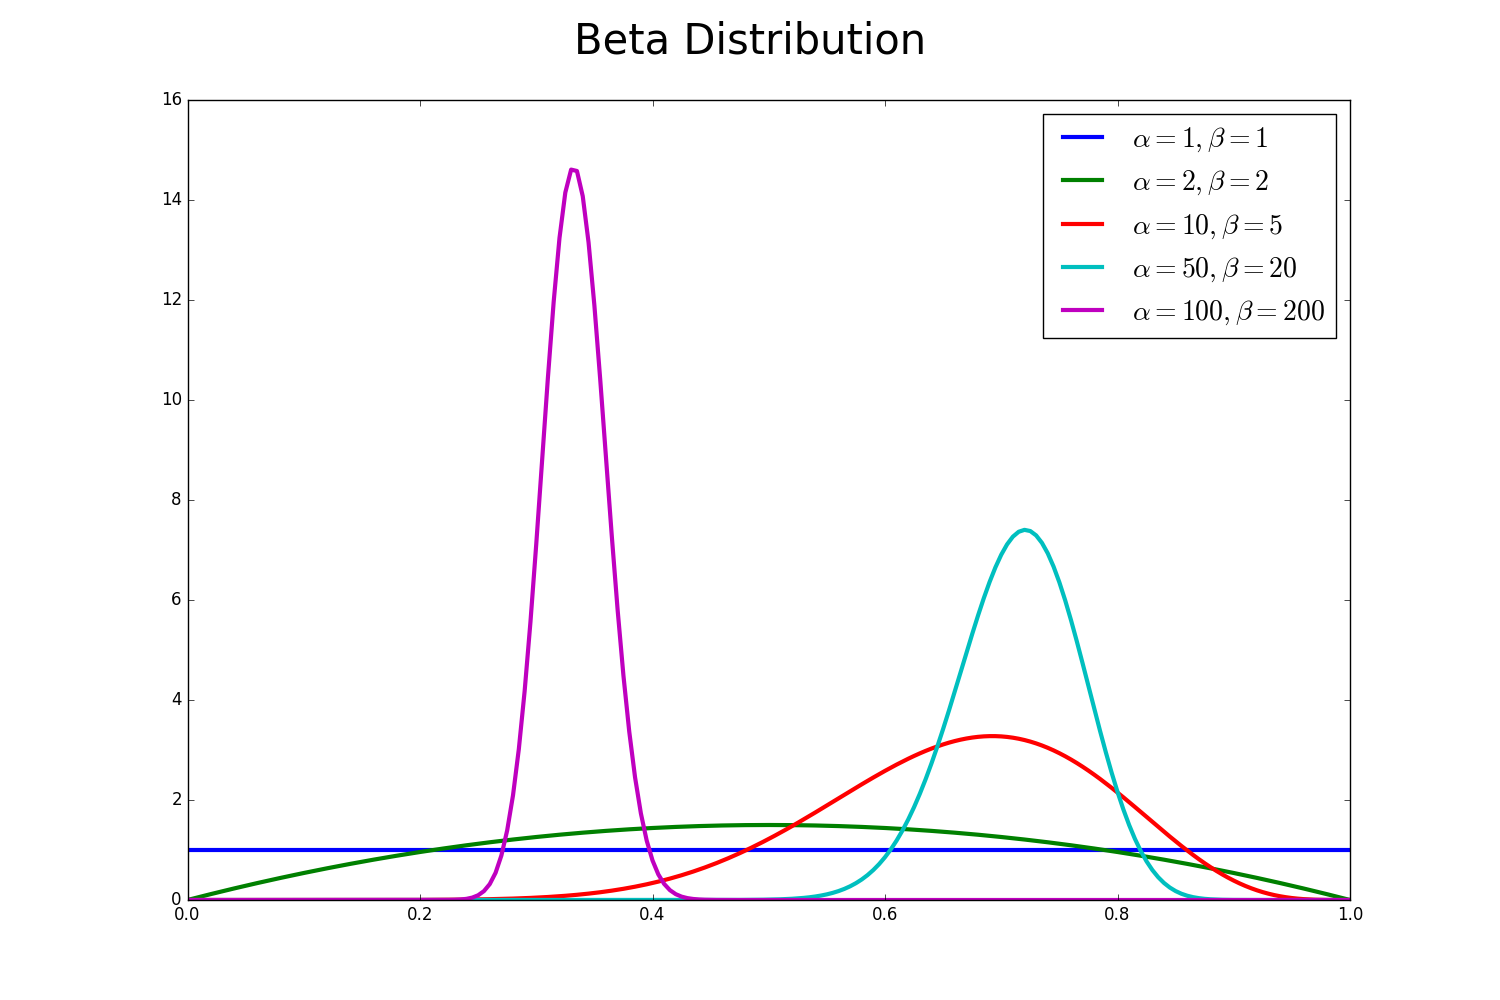
\includegraphics[width=1.2\textwidth]{images/betas.png}
      \pause

    \column{0.5\textwidth}
      \begin{itemize}
        \item {\small Choose an uninformative prior $\rightarrow \alpha = 1$ and $\beta = 1$.} \pause
        \item {\small Act like you have observed some data before that represent data your experiment has to overcome.}
      \end{itemize}
  \end{columns}
\end{frame}

\begin{frame}[fragile]
  \frametitle{Bayesian A/B Testing in Code}
  How do we actually perform a test with code, then? By simulation. \vspace{4mm}
  \begin{lstlisting}
  from numpy.random import beta

  num_samples = 10000
  alpha = beta = 1
  site_a_simulation = beta(num_conv_a + alpha,
                         num_views_a - num_conv_a + beta,
                         size=num_samples)
  site_b_simulation = beta(num_conv_b + alpha,
                         num_views_b - num_conv_b + beta,
                         size=num_samples)
  \end{lstlisting}
\end{frame}

\begin{frame}[fragile]
  \frametitle{Bayesian A/B Testing in Code Cont.}
  What's the probability that site A has a higher conversion rate than site B? \vspace{2mm}
  \begin{lstlisting}[firstnumber=11]
  np.mean(site_a_simulation > site_b_simulation)
  \end{lstlisting} \vspace{4mm}
  \pause

  What's the probability that site A has a 5\% higher conversion rate than site B? \vspace{2mm}
  \begin{lstlisting}[firstnumber=12]
  np.mean(site_a_simulation > (site_b_simulation + 0.05))
  \end{lstlisting}
\end{frame}

\begin{frame}
  \frametitle{Visualizing the Simulation}
  \begin{columns}
    \column{0.5\textwidth}
      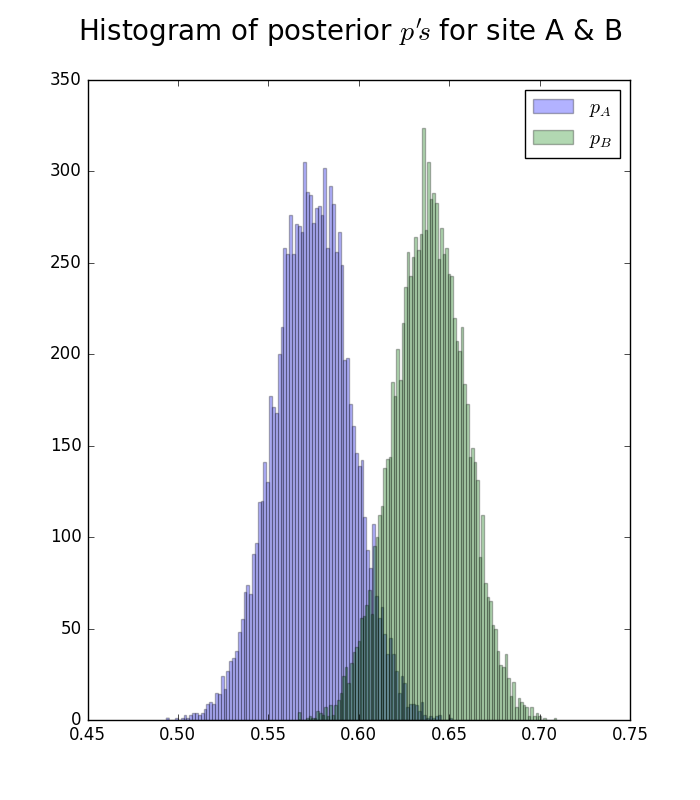
\includegraphics[width=\textwidth]{images/site_a_vs_b.png}
    \column{0.5\textwidth}
      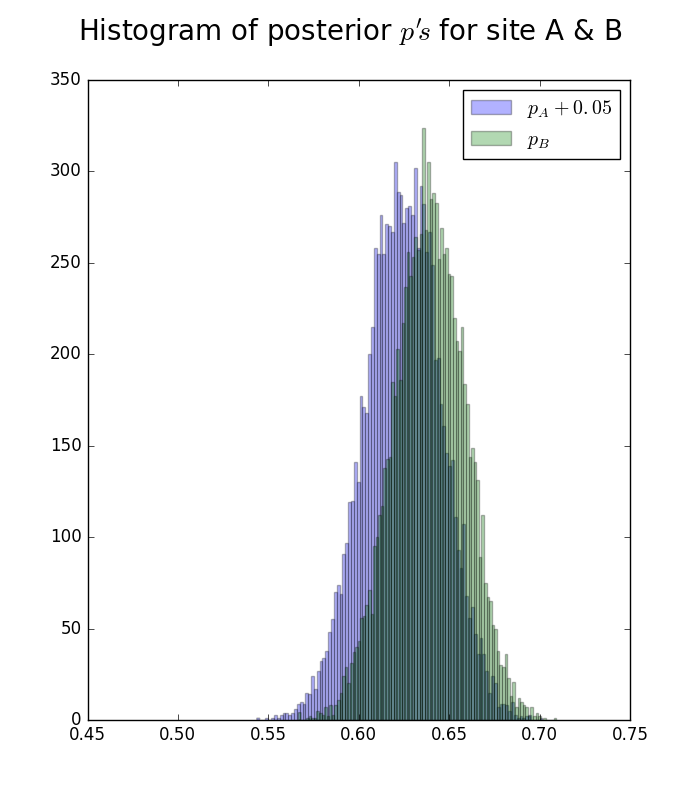
\includegraphics[width=\textwidth]{images/site_a_vs_b_5.png}
  \end{columns}
\end{frame}

\end{document}
